\documentclass{article}
% The TikZ redrawings were prepared with AI assistance.
\usepackage[en]{homework}
\usepackage{tikz}
\usepackage{needspace}
\usetikzlibrary{arrows.meta}

\tikzset{homework diagram/.style={line width=.8pt, >=Stealth, font=\normalfont\normalsize}}

\config{Physics-1}{2026 Fall}{6}

\begin{document}

\begin{problem}
A massless stick of length $b$ has one end attached to a pivot and the other end glued perpendicularly to the middle of a stick of mass $m$ and length $l$.
\begin{enumerate}
  \item[(a)] If the two sticks are held in a horizontal plane (the top figure) and then released, what is the initial acceleration of the CM?
  \item[(b)] If the two sticks are held in a vertical plane (the bottom figure) and then released, what is the initial acceleration of the CM?
\end{enumerate}
\begin{center}
  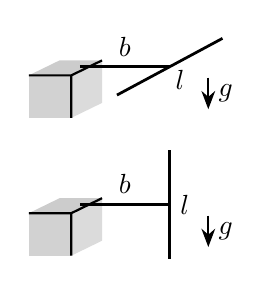
\begin{tikzpicture}[homework diagram]
  % Both views use the same projected support and pivot.
  \foreach \height in {0,1.75} {
    \begin{scope}[yshift=\height cm]
      \fill[gray!35] (0,0) rectangle (.54,-.54);
      \fill[gray!28] (.54,0) -- (.93,.19) -- (.93,-.35) -- (.54,-.54) -- cycle;
      \fill[gray!40] (0,0) -- (.39,.19) -- (.93,.19) -- (.54,0) -- cycle;
      \draw (0,0) -- (.54,0) -- (.93,.19) (.54,0) -- (.54,-.54);
      \draw[line width=1pt] (.65,.11) -- node[above] {$b$} (1.79,.11);
      \draw[->] (2.28,-.03) -- node[right] {$g$} (2.28,-.43);
    \end{scope}
  }
  \draw[line width=1pt] (1.79,-.58) -- node[right] {$l$} (1.79,.80);
  \draw[line width=1pt] (1.12,1.50) -- (2.46,2.22);
  \node at (1.92,1.69) {$l$};
\end{tikzpicture}

\end{center}
\end{problem}

\begin{solution}
	Once we have calculated the moment of inertia of the stick in both situations, say $I$, the angular acceleration is $\alpha = bmg/I$, then the acceleration is consequently $a = b\alpha = b^2mg/I$, pointing downwards vertically.

	\paragraph{(a)} The stick is parallel to the rotation axis with distance $b$, therefore $I_1 = mb^2$, then $a_1 = b^2mg/(mb^2) = g$.

	\paragraph{(b)}
	\[ I_2 = \int_{-l/2}^{l/2} (b^2 + l'^2) m/l \d l' = m \left( b^2 + \frac{l^2}{12} \right). \]
	Therefore
	\[ a_2  =\frac{b^2 mg}{I_2} = \frac{12 b^2}{12 b^2 + l^2} g. \]
\end{solution}



\begin{problem}
A uniform solid cylinder lies on top of a board. There is a friction between the two so that the cylinder does not slip. The board is placed on a table. The cylinder and the board have the same mass $m$, and the coefficient of kinetic friction between the board and the table is $\mu_k$. Initially, both the cylinder and the board have velocity $v_0$.
\begin{enumerate}
  \item[(a)] What is the acceleration of the board?
  \item[(b)] What is the speed of the cylinder when the board comes to a stop?
\end{enumerate}
\begin{center}
  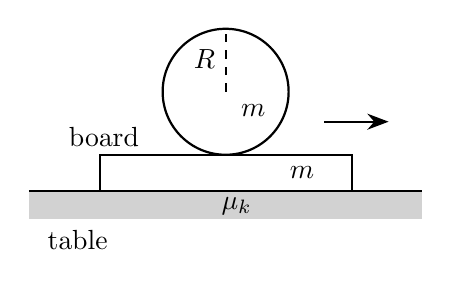
\begin{tikzpicture}[homework diagram]
  \fill[gray!35] (0,-.36) rectangle (5,0);
  \draw (0,0) -- (5,0);
  \draw (.9,0) rectangle (4.1,.46);
  \draw (2.5,1.26) circle[radius=.8];
  \draw[dashed] (2.5,1.26) -- (2.5,2.06);
  \node at (2.23,1.68) {$R$};
  \node at (2.85,1.02) {$m$};
  \node at (3.47,.23) {$m$};
  \node[anchor=east] at (1.53,.69) {board};
  \node at (.62,-.62) {table};
  \node at (2.64,-.19) {$\mu_k$};
  \draw[-{Stealth[length=2.7mm]}] (3.75,.88) -- (4.57,.88);
\end{tikzpicture}

\end{center}
\end{problem}

\begin{solution}
	This problem has already been finished in the previous homework. \textbf{(a)} The acceleration of the board has magnitude $3\mu_k g/2$ and points opposite to the initial velocity. \textbf{(b)} $v = 2v_0/3$.
\end{solution}



\begin{problem}
A uniform stick of length $l$ and mass $m$ is placed on stairs as shown below. The surface of the stairs is frictionless, except at the corner where an anti-slip tape is applied. The stick is in equilibrium. Find all forces (and their values in terms of $l$, $m$, $g$ and $\theta$) exerted on the stick.
\begin{center}
  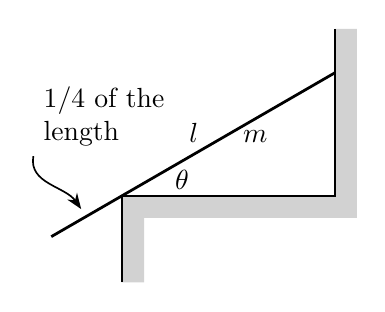
\begin{tikzpicture}[homework diagram]
  \fill[gray!35] (0,-1.10) -- (0,0) -- (2.70,0) -- (2.70,2.12)
    -- (2.98,2.12) -- (2.98,-.28) -- (.28,-.28) -- (.28,-1.10) -- cycle;
  \draw (0,-1.10) -- (0,0) -- (2.70,0) -- (2.70,2.12);
  % The stair corner is one quarter of the way along the stick.
  \draw[line width=1pt] (-.90,-.52) -- (0,0) -- (2.70,1.56);
  \node[above] at (.91,.55) {$l$};
  \node[below] at (1.69,.96) {$m$};
  \node at (.76,.20) {$\theta$};
  \node[align=left] (length) at (-.23,1.01) {1/4 of the\\length};
  \draw[->, line width=.6pt] (length.south west) to[out=-100,in=125] (-.52,-.17);
\end{tikzpicture}

\end{center}
\end{problem}

\begin{solution}
	There are three forces exerted on the stick. Gravity $mg$ points vertically downwards, the normal force $N$ at the right end points horizontally to the left, and the force at the corner is $\bo{F} = (F_x,F_y)$, with the positive directions taken to the right and upwards. Since the stick is in equilibrium,
	\[ F_x - N = 0, \qquad F_y - mg = 0. \]

	The corner is $3l/4$ from the right end. Taking torques about the right end, with counterclockwise positive, we have
	\[ \frac{l}{2}mg\cos\theta - \frac{3l}{4}F_y\cos\theta + \frac{3l}{4}F_x\sin\theta = 0. \]
	Substituting $F_y = mg$ and $F_x = N$, we get
	\[ N = F_x = \frac{mg}{3}\cot\theta, \qquad F_y = mg. \]

	Therefore, the force at the corner points upwards and to the right, with magnitude
	\[ F = mg\sqrt{1 + \frac{\cot^2\theta}{9}}, \]
	at an angle $\varphi = \arctan(3\tan\theta)$ above the horizontal.
\end{solution}



\begin{problem}
\begin{enumerate}
  \item[(a)] Compute the vector gravitational field at a point $P$ on the perpendicular bisector of the line joining two objects of equal mass separated by a distance $2a$ as shown in Figure P13.6.
  \item[(b)] Explain physically why the field should approach zero as $r \to 0$.
  \item[(c)] Prove mathematically that the answer to part (a) behaves in this way.
  \item[(d)] Explain physically why the magnitude of the field should approach $2GM/r^2$ as $r \to \infty$.
  \item[(e)] Prove mathematically that the answer to part (a) behaves correctly in this limit.
\end{enumerate}
\begin{center}
  \begin{tikzpicture}[homework diagram]
  \draw (0,-2.02) -- (0,2.02);
  \draw (-.57,0) -- (2.80,0);
  \foreach \y in {-1.52,1.52} {
    \node[circle, fill=gray!35, minimum size=5.8mm, inner sep=0pt] at (0,\y) {$M$};
    \draw[line width=.55pt] (-.57,\y) -- (-.29,\y);
    \draw[<->, line width=.55pt] (-.46,0) -- node[fill=shadecolor, inner sep=1.3pt] {$a$} (-.46,\y);
  }
  \node[below] at (1.28,0) {$r$};
  \fill (2.66,0) circle[radius=1.55pt] node[below=1pt] {$P$};
\end{tikzpicture}
\\[.4em]
  {\normalfont\bfseries Figure P13.6}
\end{center}
\end{problem}

\begin{solution}
	\paragraph{(a)} The magnitude of gravitational field at $P$ is
	\[ F(r) = 2 \frac{GM}{a^2 + r^2} \frac{r}{\sqrt{a^2 + r^2}} = \frac{2GM r}{(a^2 + r^2)^{3/2}}. \]
	Thus the vector field is $\bo{F}(\bo{r}) = -F(r)\hat{\bo{r}}$, where $\hat{\bo{r}}$ points from the midpoint to $P$.

	\paragraph{(b) (c)} The midpoint of the two objects is the equilibrium point, hence the gravitational field at this point is zero. Since the formula above is continuous at $r=0$, $\lim_{r \to 0} F(r) = F(0) = 0$.

	\paragraph{(d) (e)} When $r \gg a$, the separation of the two objects is negligible compared with their distance from $P$, so they can be regarded as a single object of mass $2M$. Hence the magnitude of the gravitational field approaches $2GM/r^2$. Mathematically,
	\[ \lim_{r \to \infty} \frac{F(r)}{2GM/r^2} = \lim_{r \to \infty} \left(1 + \frac{a^2}{r^2}\right)^{-3/2} = 1. \]
\end{solution}



\Needspace{7cm}
\begin{problem}
A sphere of matter of mass $M$ and radius $a$, has a concentric cavity of radius $b$, as shown in cross section drawn in the figure below.
\begin{enumerate}
  \item[(a)] Sketch the gravitational force $F$ exerted by the sphere on a particle of mass $m$, located a distance $r$ from the center of the sphere, as a function of $r$ in the range $0 \le r \le \infty$.
  \item[(b)] Sketch the corresponding potential energy as a function of $r$.
\end{enumerate}
\begin{center}
  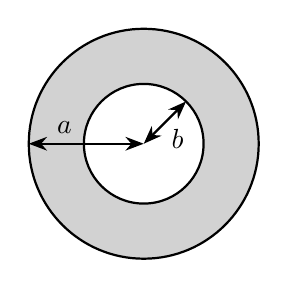
\begin{tikzpicture}[homework diagram]
  \def\outerradius{1.46}
  \def\innerradius{.76}
  \path[fill=gray!35, even odd rule]
    (0,0) circle[radius=\outerradius] circle[radius=\innerradius];
  \draw (0,0) circle[radius=\outerradius] circle[radius=\innerradius];
  \draw[<->] (-\outerradius,0) -- node[pos=.31, above] {$a$} (0,0);
  \draw[<->] (0,0) -- node[midway, below right, inner sep=2pt] {$b$} (45:\innerradius);
\end{tikzpicture}

\end{center}
\end{problem}

\begin{solution}
	\paragraph{(a)} Denote the gravitational force on the particle at $\bo{r}$ by $\bo{F}(\bo{r}) = F(r) \hat{\bo{r}}$, where $\hat{\bo{r}}$ points radially outwards. Assuming uniform density, Gauss's law gives
	\[ 4\pi r^2 F(r) = \begin{cases}
		0, & 0 \le r < b; \\
		-4 \pi GMm \frac{r^3 - b^3}{a^3 - b^3}, & b \le r < a; \\
		-4 \pi GMm, & a \le r.
	\end{cases} \]
	Therefore,
	\[ F(r) = \begin{cases}
		0, & 0 \le r < b; \\[5pt]
		-\dfrac{GMm}{a^3 - b^3}\left(r - \dfrac{b^3}{r^2}\right), & b \le r < a; \\[9pt]
		-\dfrac{GMm}{r^2}, & a \le r.
	\end{cases} \]
	The force is zero inside the cavity and points towards the center for $r>b$. Thus $F(r)$ is zero up to $r=b$, decreases to $-GMm/a^2$ at $r=a$, and then approaches zero from below as $r \to \infty$.

	\Needspace{10cm}
	\paragraph{(b)} Taking $U(\infty)=0$, the potential energy is
	\[ U(r) = \int_r^\infty F(s)\,\d s = \begin{cases}
		-\dfrac{3GMm(a^2-b^2)}{2(a^3-b^3)}, & 0 \le r < b; \\[9pt]
		-\dfrac{GMm}{2(a^3-b^3)}\left(3a^2-r^2-\dfrac{2b^3}{r}\right), & b \le r < a; \\[9pt]
		-\dfrac{GMm}{r}, & a \le r.
	\end{cases} \]
	The potential energy is constant inside the cavity and increases for $r>b$, approaching zero from below as $r \to \infty$. Both $U(r)$ and its first derivative are continuous at $r=b$ and $r=a$. The schematic plots of the force and potential energy are shown below.
	\begin{center}
		\resizebox{.46\linewidth}{!}{\begin{tikzpicture}[homework diagram, x=1cm, y=1.5cm]
  % Schematic horizontal spacing, with b at 1 and a at 2.
  \path[use as bounding box] (-2,-1.65) rectangle (6.4,.7);
  \draw[->] (0,-1.30) -- (0,.35) node[above] {$F(r)$};
  \draw[->] (0,0) -- (6,0) node[right] {$r$};
  \node[above left] at (0,0) {$0$};
  \node[above] at (1,0) {$b$};
  \node[above] at (2,0) {$a$};
  \node[left] at (0,-1) {$-\dfrac{GMm}{a^2}$};
  \draw[dashed, gray] (0,-1) -- (2,-1) -- (2,0);
  \draw[line width=1pt] (0,0) -- (1,0);
  \draw[line width=1pt, domain=1:2, samples=40]
    plot (\x,{-4*(\x-1/(\x*\x))/7});
  \draw[->, line width=1pt, domain=2:5.6, samples=60]
    plot (\x,{-4/(\x*\x)});
\end{tikzpicture}
}\hfill
		\resizebox{.46\linewidth}{!}{\begin{tikzpicture}[homework diagram, x=1cm, y=1.5cm]
  % Match the schematic horizontal spacing of the force plot.
  \path[use as bounding box] (-2,-1.65) rectangle (6.4,.7);
  \draw[->] (0,-1.55) -- (0,.35) node[above] {$U(r)$};
  \draw[->] (0,0) -- (6,0) node[right] {$r$};
  \node[above left] at (0,0) {$0$};
  \node[above] at (1,0) {$b$};
  \node[above] at (2,0) {$a$};
  \node[below left] at (0,{-9/7}) {$U(b)$};
  \node[left] at (0,-1) {$-\dfrac{GMm}{a}$};
  \draw[dashed, gray] (1,0) -- (1,{-9/7});
  \draw[dashed, gray] (0,-1) -- (2,-1) -- (2,0);
  \draw[line width=1pt] (0,{-9/7}) -- (1,{-9/7});
  \draw[line width=1pt, domain=1:2, samples=40]
    plot (\x,{-(12-\x*\x-2/\x)/7});
  \draw[->, line width=1pt, domain=2:5.6, samples=60]
    plot (\x,{-2/\x});
\end{tikzpicture}
}
	\end{center}
\end{solution}



\Needspace{12cm}
\begin{problem}
(optional) Let's inspect Descartes's Vortex theory. Imagine the universe is filled with a fluid. A star is rotating in this fluid at constant angular speed. Suppose the system has reached a steady state.

Imagine dividing the fluid into many thin spherical shells. Each shell should share the same speed rotating around the star, but this speed varies as a function of the radius away from the star.

Each shell is not accelerating or decelerating (since this is a steady state). But since these shells are moving at different speeds, they would exert a drag force on their neighbouring shells.

However, the force experienced by each shell should be vanishing. i.e. Forces tangential to the surface of each shell must cancel out.

But the velocity is changing with radius.

How do you expect the torque depends on the difference in velocities between the shells?

How do you expect the force on the surface between shells to depend on the radius of the shell.

How should the velocity scale with the radius so that the force from the outer neighbouring shell cancel with the force from the inner neighbouring shell?

Demonstrate that the period of rotation of each shell is proportional to the square of the radius of the shell -- thus contradicting astronomical observations.

Food for thought: Is it possible to fix these theory so that it matches with the observations?
\end{problem}

\end{document}
